\documentclass[a4paper,12pt]{article}

%% PACKAGES %%
\usepackage{graphicx,times,fancyhdr,algorithm,algorithmic,url}
\usepackage[left=1in,top=1in,right=1in,bottom=1in]{geometry}
\graphicspath{{./images/}}

%% DOCUMENT START %%
\begin{document}

% page numbers and headers
\thispagestyle{plain}
\pagestyle{fancy}
\clearpage
\setlength{\headsep}{0.4in}

\title{Viewed More\\ \large Measuring the effect of YouTube video title wording on view count}
%\title{Viewed More\\ \large Using NLP to Predict YouTube View Counts from Titles}
\date{\today}
\author{
  {\rm Erik Kessler and Greg Szumel}\\
  Williams College\\
  CSCI 375 \\
  Spring 2017
}

\maketitle

\lhead{CS 375}
\chead{Viewed More}
\rhead{Kessler, Szumel}
\cfoot{\thepage}

\begin{abstract}
We created a Naive Bayes classifier designed to predict whether a YouTube video is likely to receive more or less views than average for the uploader based on the title. Such a system would allow YouTube content creators to increase their view counts and would allow YouTube to increase traffic and user engagement. We created a dataset of 25k video titles from the top 1600 subscribed YouTubers. Our dataset is tagged based on the number of standard deviations away from the uploader's mean view count per video the video is. We created a variety of features including ***. We were able to achieve ***, and our classifier works best when ***. 
\end{abstract}


\section{Introduction}
Every minute, hundreds of hours of video are uploaded to YouTube. How can YouTube content creators or uploaders stand out from the crowd and draw an audience to their videos? One tool they have at their disposal is the video title. Video creators try to make their videos sound enticing by putting a flashy and interesting title to spark interest and curiosity in users with the hope the user will choose to watch their video. View counts are not only a measure of popularity but are also the main currency of YouTube as more views correspond to more opportunities for advertisements. Therefore, video creators would be interested in improving their titles to earn more money and draw more subscribers to their channel. YouTube itself is interested in keeping users on their site by making sure users continue to see interesting titles and continue to click through to those videos.

\begin{figure}[h]
    \centering
    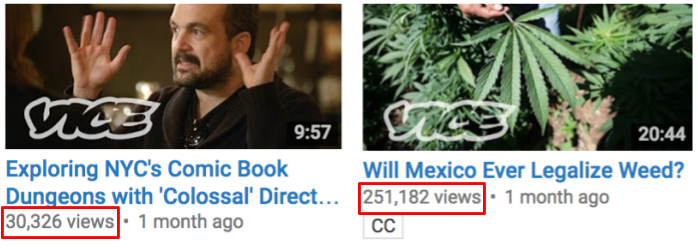
\includegraphics[width=.7\textwidth]{motivation}
    \caption{Two videos from the same uploader with drastically different view counts.}
    \label{fig:motivation}
\end{figure}

There would be value for both YouTube and video uploaders alike if when a creator uploaded a video, the site could indicate the quality of the title and even suggest a better title that would draw more views. The goal of this project was to develop a system that could predict how a video would do based on different features of the title. Such a system could also be used to filter interesting titles towards the top of search results or towards the top of a suggested videos page. Furthermore, this could be extended to detect video titles that go to far and cross into the category of clickbait which YouTube might want to filter out to avoid disappointing and annoying users.

\section{Related Work}
Our interest in this project was initially sparked by Chenhao Tan, Lillian Lee, and Bo Pang's project \textit{Retweeted More} \cite{tan+lee+pang:14}. In \textit{Retweeted More}, they developed an algorithm for predicting which of two tweets on the same topic would receive more retweets. They found that wording does matter. There are features that improve the probability that a tweet will be retweeted. This finding suggests that we will find features in YouTube title wordings that influence the number of views. We also predict that the features that improve YouTube titles will differ from those that improve tweets which is why we were interested in expanding on that project to explore YouTube. Furthermore, for this existing work, creating a dataset of content and author controlled tweets while also controlling for other confounding effects such as when the tweets were sent was a major component of the project and as they creatively used tweets-pairs from the same account linking to the same content but with different wordings as natural experiments. We would need to find or create a similar dataset for YouTube videos. \\

Existing work on determining which factors impact the popularity of YouTube videos have focused on factors such as social networks and view count histories \cite{youmna+ardon+carlsson+eager+mahanti:12}. It is difficult for a YouTuber to easily change the structure of their social network or their video's viewing patterns, so we wanted to focus on something that the uploader could easily adjust that would help them achieve more video views. Since we knew from Tan that wording had an impact on retweets and Borghol did not look at title wording, we realized we could add to existing research by studying the effect of title wording on view counts. Borghol also offered us a promising dataset of cloned videos which were sets of different re-uploads of the same video by different users. Unfortunately, many of the videos were non-English and those that were in English were movie trailers so they did not capture the types of videos on YouTube we wanted to explore. \\

Another piece of relevant work we looked at was Himabindu Lakkaraju's work on examining the effect of titles on the success of Reddit image posts \cite{himabindu+mcauley+leskovec:13}. Their finding that the title wording influences the success of a post further confirmed that wording matters, but research is missing on title wording on YouTube and what features make a good video title. Additionally, this work provides some starting points as the authors identify some linguistic features of titles that impact popularity. \\

Overall, out survey of existing work shows that wording matters, having a dataset that controls for possible confounding variables is important, and there is a current lack of literature on what features of YouTube video titles predict more popularity and views. We look to build off this existing work with our own study of wording effects on YouTube titles.


\section{Formulation}
We formulate our problem as a classification problem. We are looking to classify a string of words representing a title as either a ``good'' or ``bad'' title where good means the title will likely get more than average views and bad means the title will likely get fewer views than average. \\

To do the classification, we will construct a feature vector for the title using a variety of features that we think would be useful for predicting how a title would perform. We can then use a set of tagged feature vectors to train a classifier and use that classifier to predict the quality of unseen titles.

\section{Architecture Overview}
Provide an overview of your system, presenting and justifying important design
choices such as algorithms, features, etc.

\begin{figure}[h]
    \centering
    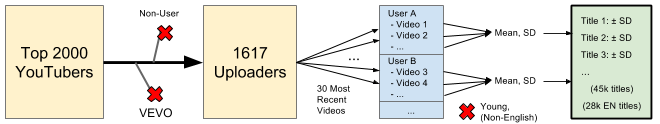
\includegraphics[width=.99\textwidth]{dataset}
    \caption{Diagram showing the dataset creation process resulting in 25k titles.}
    \label{fig:dataset}
\end{figure}


\section{Experiments \& Analysis}
Describe the dataset and the experiment setup. Compare the
performance of your system to that of a related work or other versions of your system (both if
possible!). As part of the analysis, examine the specific data points that are correctly classified by
one but not others, instead of simply focusing on the final performance scores.

\section{Limitations \& Future Work}
Summarize the project (major findings, weaknesses, etc.) and describe an extension
of the project that you’d like to try if you had more time.

\section{Conclusion}

\bibliographystyle{acm}
\bibliography{bibfile}

%\clearpage
\appendix
\section{Roles}
Describe the roles of group members.



\end{document}
